\documentclass{article}
\usepackage{amsmath}
\usepackage{xcolor}
\usepackage{tikz}
\begin{document}
\section{Live preview}
This paragraph is typeset by LuaLaTeX. Edit it and the preview follows in about a
millisecond, with inline math $e^{i\pi} + 1 = 0$ and \textcolor{blue}{colour}.

\begin{equation}\label{eq:pythagoras}
  a^2 + b^2 = c^2
\end{equation}

A second paragraph refers to equation~\eqref{eq:pythagoras} and is long enough to wrap
over two lines so that line breaking matters for the fast path of the engine.

\begin{itemize}
  \item Lists, theorems, figures and tables update as one unit.
  \item Display math such as $\sum_{k=1}^{n} k = \frac{n(n+1)}{2}$ too.
\end{itemize}

\section{An included file}
Text from an included file. Its main file is found automatically because main.tex inputs it.

\newpage
\section{A drawing}
TikZ pictures cannot be drawn from the display list, so this page is shown from the PDF of
the last full compile.

\begin{center}
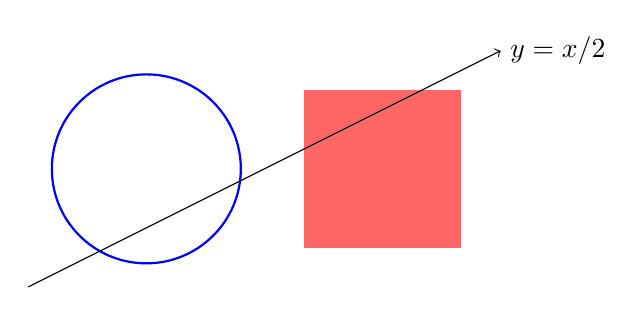
\begin{tikzpicture}
  \draw[thick,blue] (0,0) circle (1.2);
  \fill[red!60] (2,-1) rectangle (4,1);
  \draw[->] (-1.5,-1.5) -- (4.5,1.5) node[right] {$y = x/2$};
\end{tikzpicture}
\end{center}

\end{document}
